\documentclass[landscape]{article}

\pagenumbering{gobble}
\usepackage{tikz}
\usetikzlibrary{calc,shapes,positioning}
\usetikzlibrary{arrows}
\newcommand{\midarrow}{\tikz \draw[-triangle 90] (0,0) -- +(.1,0);}
\usepackage{bm}
\newcommand{\Ss}{\mathcal{S}}
\newcommand{\Tt}{\mathcal{T}}

\usepackage{amsmath,graphicx}
\newcommand{\ubar}[1]{\mkern2mu\underline{\mkern-2mu #1\mkern-2mu}\mkern2mu}
\newcommand{\ubm}[1]{\ubar{\bm{#1}}}
% \newcommand{\ubmr}[2]{\ubar{\bm{#1}}^{#2}}

\begin{document}

\begin{figure}

  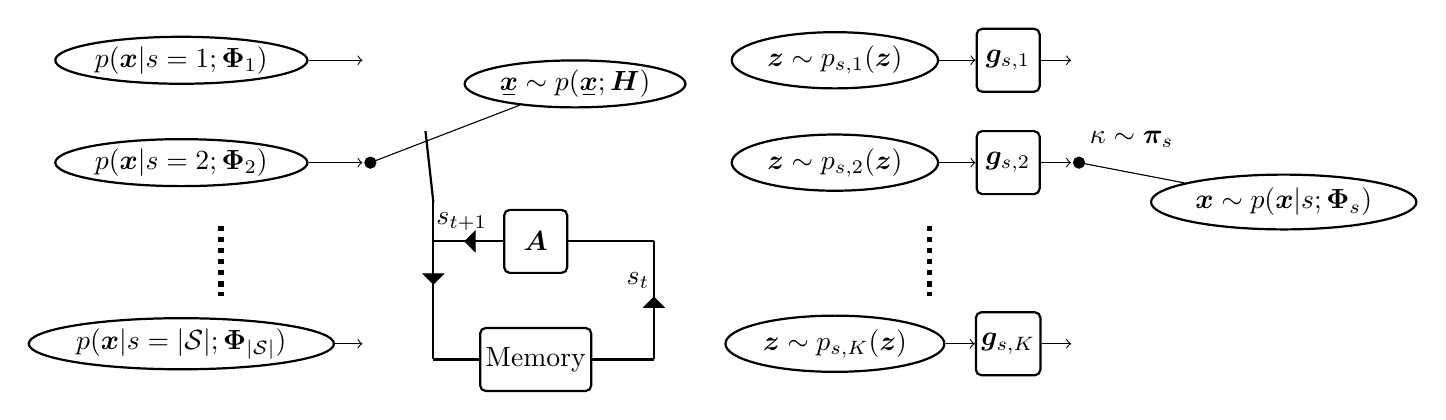
\begin{tikzpicture}


    \begin{scope}[xshift=-2cm]
      \tikzstyle{enode} = [thick, draw=black, ellipse, inner sep = 1pt,  align=center]
      \tikzstyle{nnode} = [thick, rectangle, rounded corners = 2pt,minimum size = 0.8cm,draw,inner sep = 2pt]
      \node[enode] (g1) at (-0.5,1.8) {$p(\bm{x}| s=1; \bm{\Phi}_{1})$};
      \node[enode] (g2) at (-0.5,0.5) {$p(\bm{x}| s=2; \bm{\Phi}_{2})$};
      \node[enode] (gs) at (-0.5, -1.8) {$p(\bm{x}| s=|\Ss|; \bm{\Phi}_{|\Ss|})$};
      \node[enode] (x) at (4.5,1.5){$\ubm{x}\sim p(\ubm{x};\bm{H})$};

      \draw[dotted,line width=2pt] (0,-0.3) -- (0,-1.2);
      \filldraw[->] (1.9, 0.5)circle (2pt) --  (x) ;
      \draw[->] (g1) -- (1.8, 1.8);
      \draw[->] (g2) -- (1.8, 0.5);
      \draw[->] (gs) -- (1.8, -1.8);

      \begin{scope}[xshift=0.5cm, thick, every node/.style={sloped,allow upside down}]
        \node[nnode] (m) at (3.5,-2) {Memory};
        \node[nnode] (a) at (3.5,-0.5) {$\bm{A}$};

        \draw (2.1,0.9)-- (2.2, 0.);
        \draw (2.2,0.)-- node {\midarrow} (2.2,-2);
        \draw (2.2,-2)-- (m);
        \draw (m)-- (5, -2);
        \draw (5, -2)-- node {\midarrow} (5 ,-0.5);
        \draw (5, -0.5) -- (a);
        \draw (a)-- node {\midarrow} (2.2, -0.5);
        \node at (4.8, -1) {$s_{t}$};
        \node at (2.56, -0.25) {$s_{t+1}$};
      \end{scope}
    \end{scope}


    \begin{scope}[xshift=7cm, yshift=0cm]
      \tikzstyle{enode} = [thick, draw=black, ellipse, inner sep = 2pt,  align=center]
      \tikzstyle{nnode} = [thick, rectangle, rounded corners = 2pt,minimum size = 0.8cm,draw,inner sep = 2pt]
      \node[enode] (z1) at (-1.2,1.8) {$\bm{z}\sim p_{s,1}(\bm{z})$};
      \node[nnode] (g1) at (1,1.8) {$\bm{g}_{s,1}$};
      \node[enode] (z2) at (-1.2,0.5){$\bm{z}\sim p_{s,2}(\bm{z})$};
      \node[nnode] (g2) at (1,0.5) {$\bm{g}_{s,2}$};
      \node[enode] (zK) at (-1.2,-1.8) {$\bm{z}\sim p_{s,K}(\bm{z})$};
      \node[nnode] (gs) at (1, -1.8) {$\bm{g}_{s,K}$};
      \node[enode] (x) at (4.5,0){$\bm{x}\sim p(\bm{x}| s; \bm{\Phi}_{s})$};

      \draw[dotted,line width=2pt] (0,-0.3) -- (0,-1.2);
      \filldraw[->] (1.9, 0.5)circle (2pt) --  node[above=0.2]{${\kappa}\sim \bm{\pi}_{s}$} (x)  ;
      \draw[->] (z1) -- (g1);
      \draw[->] (g1) -- (1.8, 1.8);

      \draw[->] (z2) -- (g2);
      \draw[->] (g2) -- (1.8, 0.5);

      \draw[->] (zK) -- (gs);
      \draw[->] (gs) -- (1.8, -1.8);
    \end{scope}

  \end{tikzpicture}


\end{figure}


\end{document}
%%% Local Variables:
%%% mode: latex
%%% TeX-master: t
%%% End:
